\documentclass[11pt]{article}

\usepackage[portuguese]{babel}
\usepackage[T1]{fontenc}
\usepackage[utf8]{inputenc}
\usepackage{amsmath}
\usepackage{graphicx}
\usepackage{subfig}
\usepackage[colorinlistoftodos]{todonotes}
\usepackage{listings}
\usepackage{color} 
\usepackage{float}
\usepackage[font={footnotesize}]{caption}
\usepackage{xcolor,colortbl}
\usepackage{array}
\usepackage{fixltx2e}


%lslist pra por codigo no latex?

\linespread{1.3}
\usepackage{indentfirst}
\usepackage[top=2cm, bottom=2cm, right=2.5cm, left=2.5cm]{geometry}

\begin{document}
	
\begin{titlepage}
	\begin{center}
		
		\hfill \break
		\hfill \break
		
		
\includegraphics[width=0.3\textwidth]{./logo}~\\[1cm]
		
		\textsc{\Large Mestrado Integrado em Engenharia Electrotécnica e de Computadores}\\[1.5cm]
		\textsc{\huge Sistemas Electrónicos de Processamento de Sinal}\\[0.25cm]
		
		{\huge \bfseries BPSK Modem \\[1.2cm]}
		
		Grupo n.º 2/3 \vspace{0.3cm}
		
		\begin{tabular}{l r}
			André Filipe Barroso Cerqueira \hspace{1mm} & n.º 65144 \\
			Guilherme Branco Teixeira \hspace{1mm} & n.º 70214  \\
			João André Catarino Pereira & n.º 73527
		\end{tabular}
		
		\hfill
		\hfill
		
		segunda-feira 15h30 - 18h30, LE1
		
		\vfill
		
		{\large Lisboa, 17 de Abril de 2015} 
		
	\end{center}
\end{titlepage}

\section{Índice}

\section{Introdução}

Este trabalho consiste na primeira parte do projecto de laboratório da cadeira: desenvolvimento de um modem de $Binary$ $Phase$ $Shift$ $Keying$ (BPSK). 

Teve como objectivo a familiarização com o ambiente de desenvolvimento integrado de DSP que consiste nas placas de desenvolvimento DSK TMS320C6416 e DSK TMS320C6713 da $Texas$ $Instruments$ e no software de desenvolvimento $Code Composer Studio v5.5$. Para tal correram-se dois projectos exemplo (sine8\_buf e loop\_intr) e, usando as ferramentas de debug, alteraram-se certos parâmetros de forma a observar os efeitos nos sinais resultantes. Também se consolidaram os conhecimentos adquiridos desenvolvendo dois mini projectos: um oscilador sinusoidal controlado numericamente e o modulador do modem BPSK.

%objectivo do laboratorio
%
%o que foi feito
%
%o q o relatorio vai falar

\section{Projecto}

\subsection{Projectos de Demonstração}
-Resumo das funçoes e os seus objectivos com especial importancia ao loop

-Relaciona-las com as suas utilizaçoes no projecto em si

\subsubsection{sine8\_buf}
O objectivo deste projeto é representar a função sinusoidal, multiplicada por um determinado ganho, através de um conjunto de amostras que equivalem a um período da mesma, repetindo nos períodos seguintes esse mesmo conjunto. Este procedimento é realizado através da rotina de interrupção presente no programa. 

Ao analisar o código deste projeto à primeira vista podemos concluir logo que este usa uma frequência de amostragem de 8 kHz , tem um ganho $G=10$ predefinido e usa 8 amostras para representar a sinusoide. Depois de observar a sinusoide no osciloscópio variou-se o ganho a fim de perceber a sua influência e também o seu limite.
 
Para compreender o limite desta sinusoide é necessário ter em conta que se usa o formato de vírgula fixa Q15 para as amostras da sinusoide. Este formato tem como limite o valor $(2^{15}-1) = 32767$. Considerando o valor máximo da sinusoide, se multiplicarmos a mesma por um ganho G=33 obtemos um valor superior ao permitido pelo formato Q15, fazendo com que nesses pontos o valor da sinusoide "caia".     

\subsubsection{loop\_intr}
Este projeto tem como objectivo fornecer-nos um template para os próximos projetos, em termos de comunicação com a placa e rotina de interrupção. Pode-se observar nas últimas linhas de código como se liga os sinais de entrada e saída aos canais da placa.

(comentario André)No projecto anterior observou-se os efeitos de overflow de uma variável. Neste observam-se os efeitos de aliasing(ou não, não me recordo se o DSP tem um filtro anti-aliasing à entrada)  devido ao sinal de line-in ter a mesma frequência que a frequência de amostragem. Se havia anti-aliasing, a partir dos 4khz deixariamos de ver uma sinusoide com os 3.3V. Não fizemos a experiência de mudar para sinal quadrado e variar a frequência, mas provavelmente nao iamos ver um sinal quadrado pois o espectro (infinito) deste teria que ser filtrado pelo anti-aliasing filter.

Vale a pena ir ao lab tirar esta foto?
Resultados do loop??

\subsection{BPSK}

 Demonstração dos Resultados usando como etapas as varias perguntas do enunciado, complementar com as fotos e possiveis tabelas ou partes de codigo

\subsubsection{P1. Oscilador controlado numericamente}

%fazer espectros e comparar!!!

\subsubsection{P2. Transmissor BPSK}

%Introdução Teórica
O objectivo deste projeto é criar um transmissor BPSK com recurso a três elementos principais, uma fonte de bits, um codificador diferencial e mapeador, e um modulador.
Neste projeto foi utilizada uma frequência de amostragem $f_s=16$ kHz e uma frequência portadora $f_0=4$ kHz.
%COMPLEMENTAR com alguma teoria

%Pergunta 1
Para ter uma fonte de bits no transmissor usa-se um "bit-rate clock" cuja função vai ser criar uma sequência de bits $ b_n $ que a cada 16 ciclos gera um novo bit alternado, usando um contador com $fs$/16 para determinar quando gerar um novo bit. Para alternar o bit basta negar o bit anteriormente obtido, tendo sido concretizado através de uma simples XOR:
\begin{equation}
b_n=b_{n-1} \oplus 1
\end{equation}

Após obter a fonte de bits passou-se ao segundo elemento do transmissor: o codificador diferencial e mapeador. Começando pelo codificador diferencial, este utiliza $b_n$ para aplicar a seguinte operação lógica:
\begin{equation}
c_n=c_{n-1} \oplus b_n
\end{equation}
Assim, com $c_0$ inicializado a zero codifica-se a sequência de bits $ b_n $. Ao gerar $ b_n $ e $ c_n $ obtém-se dois sinais que variam entre "0" e "1" só que $ c_n $ tem o dobro do período (figura X).
\begin{figure}[h]
	\centering
	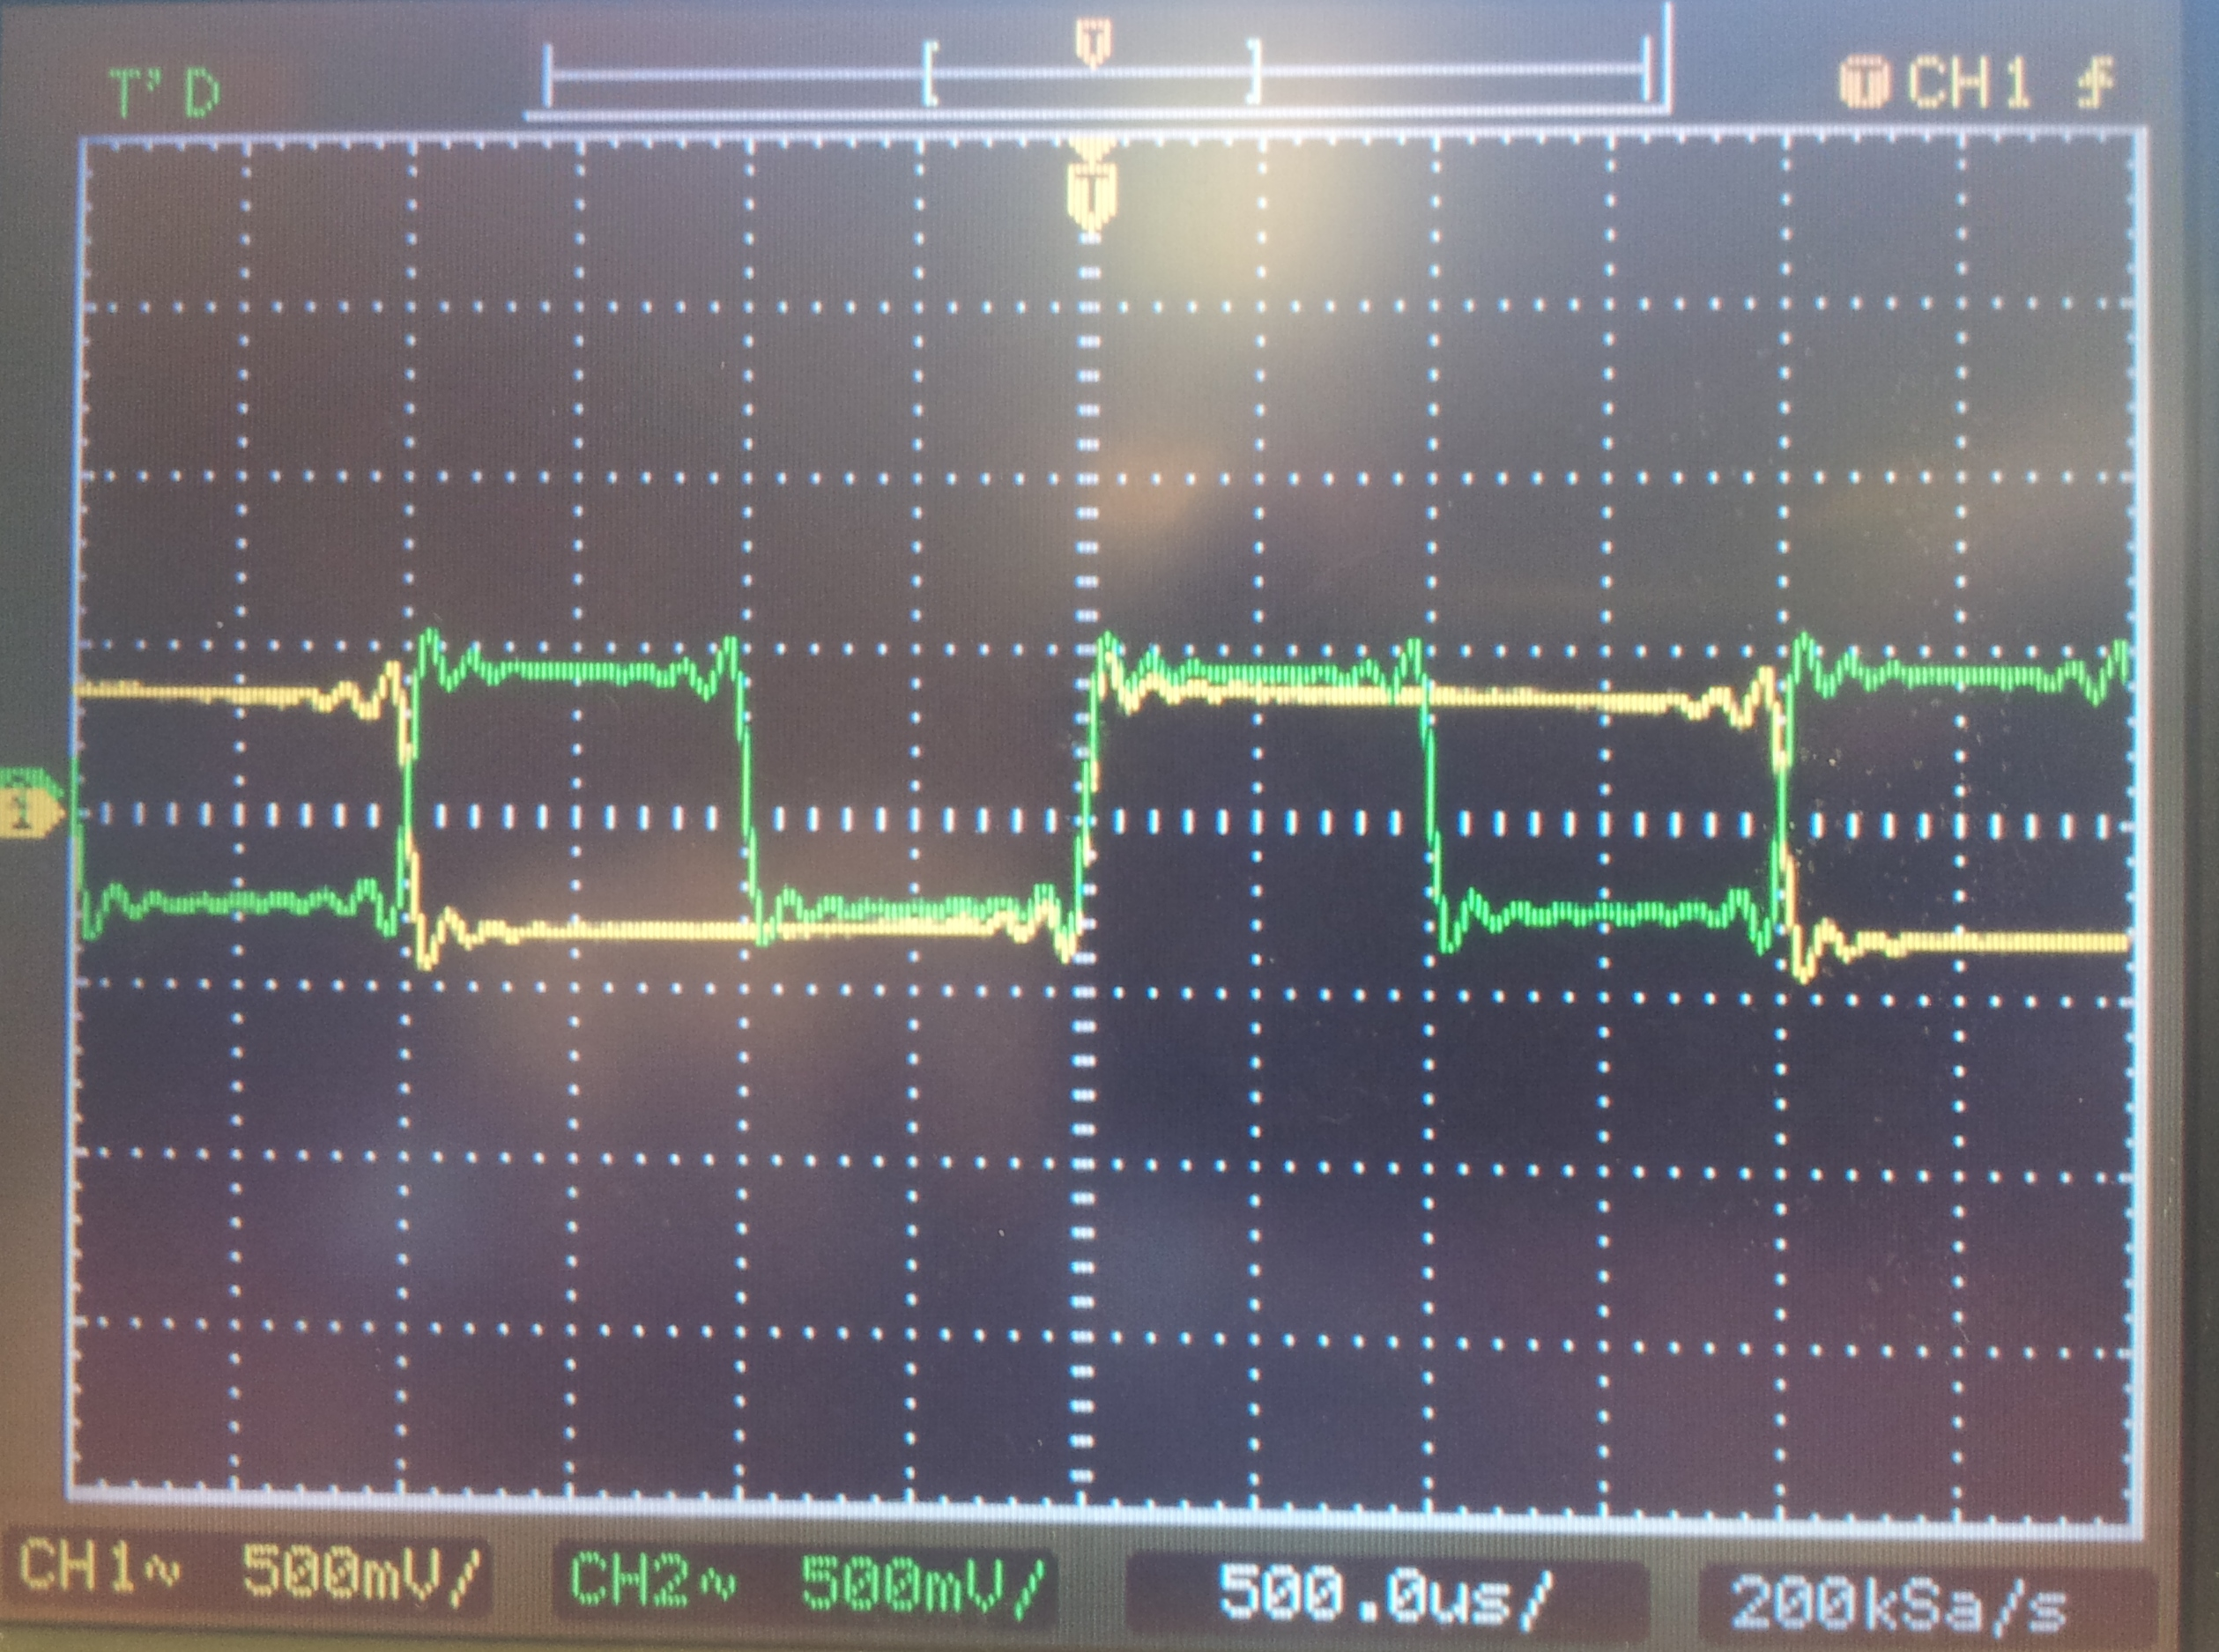
\includegraphics[width=0.5\textwidth]{./bn_cn}~\\
	\caption{$ b_n $(verde) e $ c_n $(amarelo)}
\end{figure}

%\vspace{-0.4cm} %este espaçamento dá cabo da formatação toda no meu tex.
Depois de obter $ c_n $ passa-se ao mapeamento do mesmo,
%explicar f=500Hz => uma vez que uma sequencia alternada de bits é o mesmo que uma onda quadrada, divide-se o bit rate 1kbps por dois pois cada meio ciclo da onda quadrada corresponde a um bit.
%complementar com o que?

%Pergunta 2
Falta agora gerar a onda portadora a modular. Esta foi implementada de forma mais simples face ao projeto anterior uma vez que a frequência é estática (4 kHz) e este valor consiste numa fração inteira da frequência de amostragem (16kHz).
Em primeiro lugar criou-se uma tabela com quatro valores dum período da sinusóide, sendo esta: %fazer tabela com valores

Escolheram-se estes valores uma vez que o período de amostragem coincide com os instantes de máximo, mínimo e zero-crossing da portadora. Para gerar a portadora recorreu-se a um contador que, em cada interrupção (ocorrendo em cada instante de amostragem, como explicado no enunciado), aponta para cada entrada da tabela e põe a amostra numa variável que, após se incrementar o contador, irá ser multiplicada por $d_n$. 


%Isto poderia ser mencionado na parte 1
Tem-se dois sinais Q15, ou seja o bit mais significativo para o sinal e 15 bits para a parte fracionária. Ao multiplicar-se dois sinais Q15 sabe-se que o resultado será sempre Q15
, contudo como o multiplicador retorna um valor em Q30, para este ser armazenado tem que se fazer shift left uma vez para eliminar o sinal repetido e shift right 16 vezes para transportar os bits mais significativos encostar os bits do resultado nos bits menos significativos para se truncar

% proximos 3 comments foram retirados dos slides, apagar quando quiserem:
% To store the result in a n bit word it is necessary to shift the result one bit to the left (to eliminate the replicated sign bit) and store the n MSBs of the 2n bit word
% It is possible to use a more accurate format provided the multiplication result is representable in this format (this must be known beforehand)
% Qn-1×Qn-1  can always be stored in Qn-1 because |x ·y| ≤ 1%)


%Pergunta 3

%Explicar FFT!!! 
Modulação=> tempo: é multiplicação da onda quadrada com a sinusoide. No espectro: as harmonicas ímpares (espectro quadrada) convoluídas com dirac a 4kHz(espectro portadora).
As imagens que temos retratam a onda quadrada porque não temos 4 picos como deveria ser (o espectro transladado para +- 4khz). matlab na dropbox com o espectro correcto.


\section{Conclusão}
-Principais resultados e conclusoes sobre eles, erros a corrigir (se houverem), o que melhorar

\section{Anexos}
-Codigo?

-possivelmente poe-se aqui algumas das imagens	
\end{document}